\message{ !name(5-2-real-datasets.tex)}
\message{ !name(5-2-real-datasets.tex) !offset(-2) }
In this section, we test our approximation on the Bike-Sharing
Dataset~\cite{BikeSharing}.~\footnote{It is dataset drawn from the
  Capital Bikeshare system (Washington D.C., USA) over the period
  2011-2012. The dataset can be found
  \href{https://archive.ics.uci.edu/ml/machine-learning-databases/00275/Bike-Sharing-Dataset.zip}{here}}
The Bike-Sharing Dataset is chosen as the main illustration example in
the original ALE paper, therefore we considered it appropriate for
comparisons. The dataset contains the bike rentals for almost every
hour over the period 2011 and 2012. The dataset contains 14 features,
which we denote as \( X_{\mathtt{<feature\_name>}} \). We select the
11 features that are relevant to the prediction task. Most of the
features are measurements of the environmental conditions, e.g.
\(X_{\mathtt{month}}\), \(X_{\mathtt{hour}}\),
\(X_{\mathtt{temperature}}\), \(X_{\mathtt{humidity}}\),
\(X_{\mathtt{windspeed}}\), while some others inform us about the
day-type, e.g. whether we refer to a working-day
\(X_{\mathtt{workingday}}\). The target value \( Y_{\mathtt{count}}\)
is the bike rentals per hour, which has mean value
\(\mu_{\mathtt{count}} = 189\) and standard deviation
\(\sigma_{\mathtt{count}} = 181\). We train a deep fully-connected
Neural Network with 6 hidden layers and \(711681\) parameters. We
train the model for \(20\) epochs, using the Adam optimizer with
learning rate 0.01. The model achieves a mean absolute error on the
test of about \(38\) counts.

\paragraph{Efficiency} For comparing the efficiency, we measure the
execution time of DALE and ALE for a variable number of features. We
present the results in Table~\ref{tab:bike-sharing-efficiency}. We
confirm that DALE can compute the feature effect for all features in
almost constant time wrt \(D\). In contrast, ALE scales linearly wrt
\(D\) which leads to an execution time of over \(10\) seconds even for
our dataset with 14 features.

\begin{table}
  \centering
  \begin{tabular}{c|c|c|c|c|c|c|c|c|c|c|c}
    \multicolumn{12}{c}{Efficiency} \\
    \hline\hline
    & \multicolumn{11}{|c}{Number of Features} \\
    \hline
    & 1 & 2 & 3 & 4 & 5 & 6 & 7 & 8 & 9 & 10 & 11 \\
    \hline
    \( \dale \) & 1.17 & 1.19 & 1.22 & 1.24 & 1.27 & 1.30 & 1.36 & 1.32 & 1.33 & 1.37 & 1.39 \\
    \hline
    \( \alep \) & 0.85 & 1.78 & 2.69 & 3.66 & 4.64 & 5.64 & 6.85 & 7.73 & 8.86 & 9.9 & 10.9 \\
    \hline
  \end{tabular}
  \caption{Evaluation of the divergence between DALE and ALE
    estimation on the Bike Sharing dataset.}
  \label{tab:bike-sharing-efficiency}
\end{table}

\paragraph{Accuracy}

In the case of the bike-sharing, it is infeasible to compute the
ground-truth ALE.~Firstly, we have lack of knowledge about the
data-generating distribution and, secondly, the dimensionality of the
problem \(D=14\) is prohibiting for applying numerical integration on
eq.~\eqref{eq:ALE}. However, exploiting that the dataset is very
dense, we can treat DALE and ALE approximation as ground truth effect.

Afterwards, to simulate the case of sparse dataset and recompute the
effect with we can artificially


contains enough samples, we can split the axis of each feature
in dense bins, i.e. large \(K\),

and treat the ALE apporoximation as the ground truth
effect.

In Table~\ref{tab:bike-sharing} we present the MSE between ALE
and DALE and in Figure~\ref{fig:bike-sharing-comparison} (a), (b),
(c), we illustrate the approximations in three features. In all cases,
DALE provides almost identical estimates to ALE, i.e., NMSE less than
\(10^{-3}\). Therefore, we can confirm that in cases of dense samples,
DALE is a much faster and equally-accurate alternative to ALE
approximation.

\begin{figure}[h]
  \begin{center}
    \begin{tabular}{cccc}
      \resizebox{.22\columnwidth}{!}{% This file was created with tikzplotlib v0.10.1.
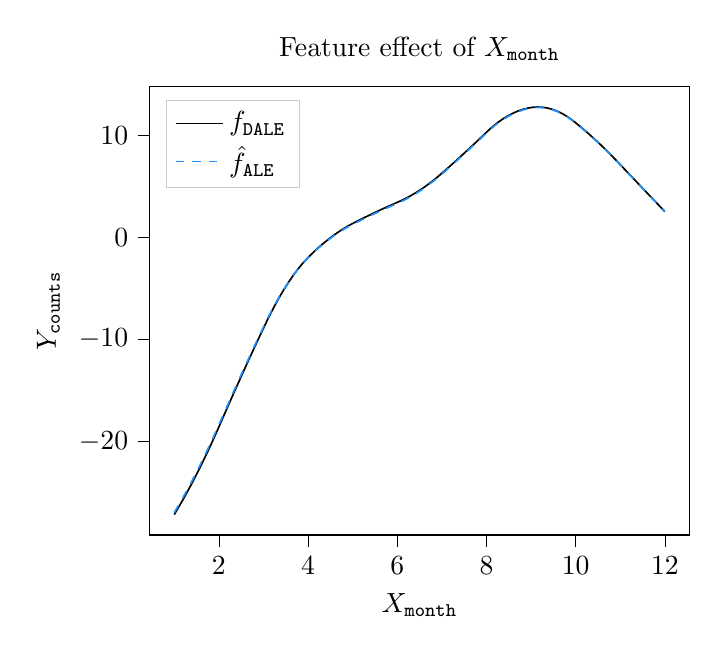
\begin{tikzpicture}

\definecolor{darkgray176}{RGB}{176,176,176}
\definecolor{dodgerblue}{RGB}{30,144,255}
\definecolor{lightgray204}{RGB}{204,204,204}

\begin{axis}[
legend cell align={left},
legend style={
  fill opacity=0.8,
  draw opacity=1,
  text opacity=1,
  at={(0.03,0.97)},
  anchor=north west,
  draw=lightgray204
},
tick align=outside,
tick pos=left,
title={Feature effect of \(\displaystyle X_{\mathtt{month}}\)},
x grid style={darkgray176},
xlabel={\(\displaystyle X_{\mathtt{month}}\)},
xmin=0.45, xmax=12.55,
xtick style={color=black},
y grid style={darkgray176},
ylabel={\(\displaystyle Y_{\mathtt{counts}}\)},
ymin=-29.183798458369, ymax=14.7468616660552,
ytick style={color=black}
]
\addplot [semithick, black]
table {%
1 -27.1869506835938
1.17617619037628 -25.871150970459
1.29729723930359 -24.9201946258545
1.40740740299225 -24.0201549530029
1.51751756668091 -23.0867099761963
1.63863861560822 -22.0221939086914
1.74874877929688 -21.0186061859131
1.85885882377625 -19.9816131591797
1.9689689874649 -18.9112167358398
2.09009003639221 -17.6963996887207
2.32132124900818 -15.3969707489014
2.64064073562622 -12.2988424301147
2.87187194824219 -10.1101322174072
3.1141140460968 -7.87898731231689
3.24624633789062 -6.75733757019043
3.35635638237 -5.88665103912354
3.45545554161072 -5.15343141555786
3.56556558609009 -4.3964409828186
3.67567563056946 -3.69928789138794
3.77477478981018 -3.12166857719421
3.88488483428955 -2.53821158409119
3.99499487876892 -2.01459169387817
4.13813829421997 -1.40747404098511
4.23723745346069 -1.0118283033371
4.34734725952148 -0.59662914276123
4.45745754241943 -0.207057595252991
4.56756734848022 0.156886339187622
4.66666650772095 0.462822675704956
4.7767767906189 0.778071641921997
4.88688707351685 1.06769299507141
4.98598575592041 1.30698728561401
5.21721744537354 1.81831657886505
5.43743753433228 2.28735709190369
5.64664649963379 2.71674489974976
5.86686706542969 3.15148568153381
6.12012004852295 3.64487433433533
6.19719696044922 3.81250214576721
6.30730724334717 4.07315158843994
6.42842864990234 4.38769626617432
6.53853845596313 4.69808197021484
6.64864873886108 5.03215312957764
6.75875854492188 5.3899097442627
6.87987995147705 5.81102657318115
6.98998975753784 6.21852016448975
7.23223209381104 7.15501070022583
7.463463306427 8.071533203125
7.6836838722229 8.96508026123047
7.90390396118164 9.87869548797607
8.09109115600586 10.6491012573242
8.17917919158936 10.9760904312134
8.27827835083008 11.3111982345581
8.38838863372803 11.6416292190552
8.49849891662598 11.9293622970581
8.60860824584961 12.1743965148926
8.70770740509033 12.3600397109985
8.81781768798828 12.5239429473877
8.92792797088623 12.6451482772827
9.03803825378418 12.7230014801025
9.1371374130249 12.7500133514404
9.17016983032227 12.7448768615723
9.24724769592285 12.7297611236572
9.28028011322021 12.7090911865234
9.35735702514648 12.6578493118286
9.40140151977539 12.6091642379761
9.47847843170166 12.5178241729736
9.58858871459961 12.3373823165894
9.69869899749756 12.1052808761597
9.80880928039551 11.8215208053589
9.92992973327637 11.4478168487549
10.1061058044434 10.8241405487061
10.2162160873413 10.4159374237061
10.3263263702393 9.99349880218506
10.4364366531372 9.55682373046875
10.5575571060181 9.06051921844482
10.667667388916 8.59395122528076
10.777777671814 8.11314868927002
10.8988990783691 7.56844854354858
11.7247247695923 3.76278614997864
12 2.50704598426819
};
\addlegendentry{$f_{\mathtt{DALE}}$}
\addplot [semithick, dodgerblue, dashed]
table {%
1 -27.0010604858398
1.18718719482422 -25.586950302124
1.29729723930359 -24.7142314910889
1.40740740299225 -23.809778213501
1.52852857112885 -22.77903175354
1.63863861560822 -21.8079357147217
1.74874877929688 -20.8051052093506
1.86986982822418 -19.666467666626
1.99099099636078 -18.4894695281982
2.2992992401123 -15.4285402297974
2.51951956748962 -13.2975368499756
2.72872877120972 -11.3166017532349
2.94894886016846 -9.27656745910645
3.1141140460968 -7.78738117218018
3.24624633789062 -6.68413352966309
3.35635638237 -5.82812023162842
3.45545554161072 -5.10758543014526
3.56556558609009 -4.36409330368042
3.67567563056946 -3.67981958389282
3.77477478981018 -3.113276720047
3.88488483428955 -2.54152417182922
3.99499487876892 -2.02899026870728
4.13813829421997 -1.43530428409576
4.23723745346069 -1.04830312728882
4.34734725952148 -0.642061471939087
4.45745754241943 -0.260767459869385
4.56756734848022 0.0955789089202881
4.66666650772095 0.395250797271729
4.7767767906189 0.704194068908691
4.88688707351685 0.988189816474915
4.98598575592041 1.22298789024353
5.23923921585083 1.77311503887177
5.4484486579895 2.21300554275513
5.66866874694824 2.66170525550842
5.88888883590698 3.09569883346558
6.10910892486572 3.52712678909302
6.19719696044922 3.71933627128601
6.30730724334717 3.9817156791687
6.42842864990234 4.29802989959717
6.53853845596313 4.60990715026855
6.64864873886108 4.9453558921814
6.75875854492188 5.30437612533569
6.87987995147705 5.72675085067749
6.98998975753784 6.13526916503906
7.24324321746826 7.11681127548218
7.463463306427 7.99168014526367
7.6836838722229 8.8862886428833
7.90390396118164 9.80063629150391
8.09109115600586 10.5716905593872
8.17917919158936 10.899432182312
8.2892894744873 11.2697401046753
8.38838863372803 11.5681610107422
8.49849891662598 11.8583631515503
8.60860824584961 12.106406211853
8.70770740509033 12.2951984405518
8.81781768798828 12.463134765625
8.92792797088623 12.5889139175415
9.03803825378418 12.6718053817749
9.1371374130249 12.702956199646
9.17016983032227 12.6990699768066
9.24724769592285 12.6868410110474
9.28028011322021 12.6672773361206
9.35735702514648 12.6185913085938
9.40140151977539 12.5711889266968
9.47847843170166 12.4820346832275
9.58858871459961 12.3042573928833
9.69869899749756 12.0743465423584
9.80880928039551 11.7923011779785
9.92992973327637 11.4199190139771
10.1061058044434 10.7974834442139
10.2162160873413 10.3899793624878
10.3263263702393 9.96817970275879
10.4364366531372 9.53208541870117
10.5575571060181 9.03635120391846
10.667667388916 8.57023906707764
10.777777671814 8.08983135223389
10.8988990783691 7.54549980163574
11.7027025222778 3.84338307380676
12 2.48848509788513
};
\addlegendentry{$\hat{f}_{\mathtt{ALE}}$}
\end{axis}

\end{tikzpicture}
}&
      \resizebox{.22\columnwidth}{!}{% This file was created with tikzplotlib v0.10.1.
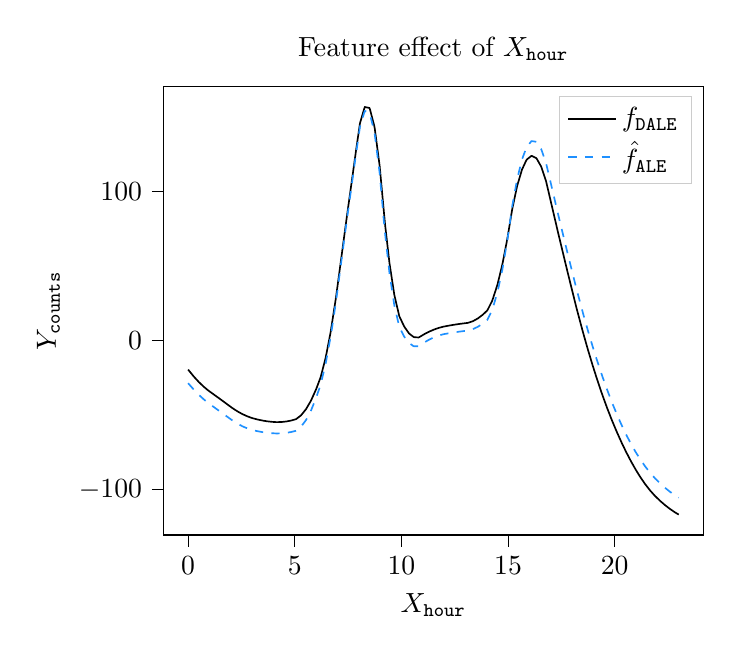
\begin{tikzpicture}

\definecolor{darkgray176}{RGB}{176,176,176}
\definecolor{dodgerblue}{RGB}{30,144,255}
\definecolor{lightgray204}{RGB}{204,204,204}

\begin{axis}[
legend cell align={left},
legend style={fill opacity=0.8, draw opacity=1, text opacity=1, draw=lightgray204},
tick align=outside,
tick pos=left,
title={Feature effect of \(\displaystyle X_{\mathtt{hour}}\)},
x grid style={darkgray176},
xlabel={\(\displaystyle X_{\mathtt{hour}}\)},
xmin=-1.15, xmax=24.15,
xtick style={color=black},
y grid style={darkgray176},
ylabel={\(\displaystyle Y_{\mathtt{counts}}\)},
ymin=-130.55351264475, ymax=170.472616656964,
ytick style={color=black}
]
\addplot [semithick, black]
table {%
0 -19.5050849914551
0.276276350021362 -24.3441772460938
0.506506443023682 -27.9236030578613
0.73673677444458 -31.0645523071289
0.943943977355957 -33.5316467285156
1.54254257678986 -39.7169952392578
2.00300312042236 -44.5988159179688
2.11811804771423 -45.7644081115723
2.32532525062561 -47.663459777832
2.55555558204651 -49.4630393981934
2.78578567504883 -50.9483070373535
2.99299287796021 -52.0300178527832
3.24624633789062 -52.9924545288086
3.47647643089294 -53.6967239379883
3.68368363380432 -54.1934471130371
3.91391396522522 -54.5767364501953
4.14414405822754 -54.7889671325684
4.37437438964844 -54.7139015197754
4.60460472106934 -54.3515357971191
4.83483505249023 -53.7018775939941
5.04204225540161 -52.8642959594727
5.06506490707397 -52.7370185852051
5.29529523849487 -50.2154121398926
5.52552556991577 -46.1370544433594
5.75575590133667 -40.5019493103027
6.00900888442993 -32.4394378662109
6.21621608734131 -24.4946517944336
6.44644641876221 -11.6443128585815
6.67667675018311 5.24092245101929
6.92992973327637 28.6440601348877
7.43643665313721 82.6207962036133
7.89689683914185 130.067947387695
8.05805778503418 145.936157226562
8.26526546478271 156.092514038086
8.28828811645508 156.789611816406
8.49549579620361 156.161087036133
8.51851844787598 155.647872924805
8.72572612762451 144.234481811523
8.74874877929688 142.510955810547
8.97897911071777 117.378860473633
9.23223209381104 78.1012954711914
9.43943977355957 52.0760345458984
9.66967010498047 30.5269412994385
9.89989948272705 16.3793964385986
10.1301298141479 9.40791988372803
10.3603601455688 4.70836496353149
10.5675678253174 2.42953133583069
10.5905904769897 2.28073143959045
10.7977981567383 2.04458355903625
10.8208208084106 2.12501859664917
11.0740737915039 4.29217100143433
11.3043041229248 5.98237943649292
11.5345344543457 7.39637041091919
11.7417421340942 8.44379425048828
11.9719715118408 9.33294486999512
12.2482481002808 10.0710592269897
12.4784784317017 10.624490737915
12.7087087631226 11.1187515258789
12.9159154891968 11.5147294998169
13.1001005172729 11.8276166915894
13.1231231689453 11.9058475494385
13.3303298950195 12.875524520874
13.3763761520386 13.199444770813
13.5835838317871 14.8272914886475
13.813814163208 17.3185062408447
14.0210208892822 20.1412181854248
14.0670671463013 21.3190975189209
14.2512512207031 26.5641231536865
14.2972974777222 28.4294090270996
14.5045042037964 37.6234588623047
14.7347345352173 51.2384872436523
14.9649648666382 68.2768707275391
15.1951951980591 88.2222595214844
15.42542552948 103.759735107422
15.6556558609009 114.889282226562
15.8628625869751 121.212203979492
15.8858861923218 121.610908508301
16.0930938720703 123.970664978027
16.1161155700684 123.936637878418
16.3233242034912 122.487854003906
16.3693695068359 121.442276000977
16.5535526275635 116.769096374512
16.6226234436035 113.865631103516
16.7837829589844 106.814399719238
16.8758754730225 101.206695556641
17.3363361358643 72.9654541015625
17.7967967987061 45.5679664611816
18.2112121582031 21.7020950317383
18.5105113983154 5.64360857009888
18.7407398223877 -5.97945785522461
18.9709701538086 -16.9456024169922
19.1781787872314 -26.2628364562988
19.4084091186523 -35.9988479614258
19.6386394500732 -45.0910110473633
19.8688697814941 -53.5393295288086
20.0990982055664 -61.3896484375
20.3293285369873 -68.7146987915039
20.5365371704102 -74.8665542602539
20.7667675018311 -81.1935348510742
20.996997833252 -86.995246887207
21.2042045593262 -91.7762222290039
21.4344348907471 -96.5489959716797
21.664665222168 -100.770584106445
21.8948955535889 -104.44100189209
22.1481475830078 -107.900184631348
22.3553562164307 -110.46851348877
22.5855846405029 -113.02222442627
22.8158149719238 -115.269233703613
23 -116.870506286621
};
\addlegendentry{$f_{\mathtt{DALE}}$}
\addplot [semithick, dodgerblue, dashed]
table {%
0 -28.6461296081543
0.299299240112305 -33.4844398498535
0.506506443023682 -36.5122833251953
0.73673677444458 -39.5242080688477
0.966966986656189 -42.1757049560547
1.74974977970123 -50.2825317382812
2.11811804771423 -54.0799827575684
2.32532525062561 -55.9247512817383
2.55555558204651 -57.6483955383301
2.78578567504883 -59.0419044494629
2.99299287796021 -60.0281982421875
3.24624633789062 -60.8593711853027
3.47647643089294 -61.46630859375
3.68368363380432 -61.8931121826172
3.91391396522522 -62.2204475402832
4.14414405822754 -62.3986968994141
4.37437438964844 -62.3219032287598
4.60460472106934 -61.990062713623
4.83483505249023 -61.4031791687012
5.04204225540161 -60.6504898071289
5.06506490707397 -60.5277214050293
5.29529523849487 -57.8714256286621
5.52552556991577 -53.4342956542969
5.75575590133667 -47.2163352966309
6.00900888442993 -38.2443809509277
6.21621608734131 -29.381742477417
6.44644641876221 -15.6827802658081
6.69969987869263 4.01029825210571
6.92992973327637 25.8215217590332
7.39039039611816 75.5200271606445
7.85085105895996 123.192329406738
8.05805778503418 143.596130371094
8.26526546478271 153.462203979492
8.28828811645508 154.119873046875
8.49549579620361 153.021850585938
8.51851844787598 152.449096679688
8.72572612762451 140.386978149414
8.74874877929688 138.58381652832
8.97897911071777 112.524017333984
9.20920944213867 75.0672760009766
9.43943977355957 45.3751182556152
9.66967010498047 23.4475517272949
9.89989948272705 9.28457546234131
10.1301298141479 2.64411807060242
10.3603601455688 -1.73881900310516
10.5675678253174 -3.74506211280823
10.5905904769897 -3.86423587799072
10.7977981567383 -3.84074091911316
10.8208208084106 -3.73213291168213
11.0740737915039 -1.27214574813843
11.3043041229248 0.624772906303406
11.5115118026733 2.059002161026
11.7417421340942 3.31951761245728
11.9719715118408 4.24510145187378
12.2482481002808 4.96000051498413
12.4784784317017 5.49322175979614
12.7087087631226 5.96644258499146
12.9159154891968 6.34280109405518
13.1001005172729 6.63770151138306
13.1231231689453 6.70726346969604
13.3303298950195 7.55532884597778
13.3763761520386 7.83442735671997
13.5835838317871 9.23264122009277
13.813814163208 11.3566951751709
14.0210208892822 13.7536668777466
14.0440444946289 14.2715625762939
14.2512512207031 20.38014793396
14.2972974777222 22.4057006835938
14.5045042037964 32.4857139587402
14.7347345352173 47.7849960327148
14.9649648666382 67.2124176025391
15.1951951980591 90.178352355957
15.42542552948 108.329772949219
15.6556558609009 121.666687011719
15.8628625869751 129.635528564453
15.9089088439941 130.593536376953
16.0930938720703 133.829193115234
16.1161155700684 133.91423034668
16.3233242034912 133.447540283203
16.3463459014893 133.071701049805
16.5535526275635 128.498184204102
16.5995998382568 126.696998596191
16.7837829589844 118.981163024902
16.8758754730225 113.421195983887
17.3363361358643 85.3754196166992
17.7967967987061 58.1768074035645
18.2112121582031 34.4831466674805
18.5335330963135 17.2674236297607
18.7407398223877 6.80826711654663
18.9709701538086 -4.24147033691406
19.2012004852295 -14.6806631088257
19.4084091186523 -23.5517692565918
19.6386394500732 -32.8170890808105
19.8688697814941 -41.4646186828613
20.0990982055664 -49.5049858093262
20.3063068389893 -56.2461433410645
20.5365371704102 -63.1648941040039
20.7667675018311 -69.4933547973633
20.9739742279053 -74.6995239257812
21.2272281646729 -80.4064331054688
21.4344348907471 -84.651123046875
21.664665222168 -88.8804550170898
21.8948955535889 -92.6121520996094
22.1481475830078 -96.1844940185547
22.3553562164307 -98.8407440185547
22.5855846405029 -101.486793518066
22.8158149719238 -103.820686340332
23 -105.487968444824
};
\addlegendentry{$\hat{f}_{\mathtt{ALE}}$}
\end{axis}

\end{tikzpicture}
}&
      \resizebox{.22\columnwidth}{!}{% This file was created with tikzplotlib v0.10.1.
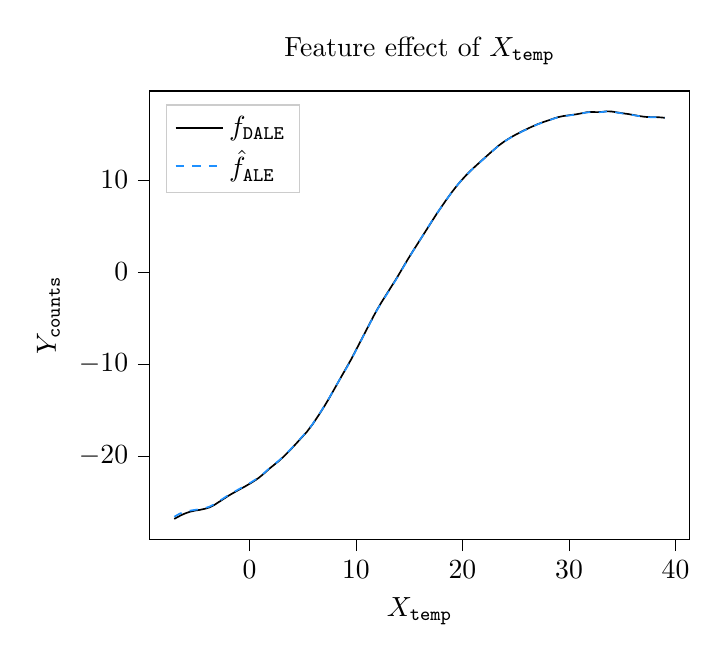
\begin{tikzpicture}

\definecolor{darkgray176}{RGB}{176,176,176}
\definecolor{dodgerblue}{RGB}{30,144,255}
\definecolor{lightgray204}{RGB}{204,204,204}

\begin{axis}[
legend cell align={left},
legend style={
  fill opacity=0.8,
  draw opacity=1,
  text opacity=1,
  at={(0.03,0.97)},
  anchor=north west,
  draw=lightgray204
},
tick align=outside,
tick pos=left,
title={Feature effect of \(\displaystyle X_{\mathtt{temp}}\)},
x grid style={darkgray176},
xlabel={\(\displaystyle X_{\mathtt{temp}}\)},
xmin=-9.363, xmax=41.303,
xtick style={color=black},
y grid style={darkgray176},
ylabel={\(\displaystyle Y_{\mathtt{counts}}\)},
ymin=-29.0709646178484, ymax=19.6587744022419,
ytick style={color=black}
]
\addplot [semithick, black]
table {%
-7.05999994277954 -26.8559761047363
-6.46062040328979 -26.4800567626953
-6.0456657409668 -26.2643947601318
-5.58460474014282 -26.0768356323242
-5.12354373931885 -25.9551944732666
-4.6163763999939 -25.8672676086426
-4.15531539916992 -25.7476043701172
-3.78646636009216 -25.6194591522217
-3.32540535926819 -25.3593654632568
-1.89611613750458 -24.2860908508301
-1.29673671722412 -23.8906536102295
-0.374614596366882 -23.3033409118652
0.13255250453949 -22.9581642150879
0.593613624572754 -22.6199989318848
0.870250225067139 -22.3956699371338
1.3313113451004 -21.958179473877
1.88458454608917 -21.3814105987549
2.34564566612244 -20.9465732574463
2.71449446678162 -20.6056251525879
3.17555546760559 -20.1241321563721
3.86714720726013 -19.3148040771484
4.32820844650269 -18.7428874969482
5.38864850997925 -17.393705368042
5.94192171096802 -16.5494594573975
6.54130125045776 -15.5111389160156
7.04846858978271 -14.5789861679077
7.46342325210571 -13.7732734680176
7.92448425292969 -12.8301782608032
8.56997013092041 -11.506103515625
9.53819847106934 -9.53578948974609
11.6590795516968 -4.80234098434448
11.981822013855 -4.11864328384399
12.3967771530151 -3.30403637886047
13.8260660171509 -0.680456161499023
14.4254455566406 0.496161341667175
14.8865060806274 1.39492416381836
15.3475675582886 2.25227308273315
17.560661315918 6.27518367767334
18.4366760253906 7.75337982177734
18.9438438415527 8.56881618499756
19.4049053192139 9.25801277160645
19.819860458374 9.83408832550049
20.2809200286865 10.4210844039917
20.8341941833496 11.064582824707
21.2952556610107 11.5648498535156
22.6784381866455 13.0035104751587
23.3700294494629 13.6961889266968
23.923303604126 14.1664371490479
24.4765758514404 14.5691957473755
24.9376373291016 14.8722658157349
25.6292285919189 15.2886924743652
26.4130325317383 15.7198438644409
27.0585193634033 16.0503673553467
27.6578979492188 16.3048324584961
28.6722316741943 16.7012271881104
28.9488697052002 16.8027153015137
29.4099292755127 16.9200115203857
30.7470073699951 17.1318607330322
31.4385986328125 17.2897148132324
31.6691284179688 17.3425445556641
32.1301918029785 17.378532409668
32.6373558044434 17.3518009185791
33.0984191894531 17.3830833435059
33.5133743286133 17.4437866210938
33.9744338989258 17.4278163909912
34.8504486083984 17.2642993927002
35.6342544555664 17.1358203887939
36.0492095947266 17.045431137085
36.5563774108887 16.9395217895508
37.0174369812012 16.8616962432861
37.294075012207 16.8304462432861
37.7551345825195 16.8116798400879
38.2161979675293 16.8119583129883
38.6772575378418 16.7783241271973
39 16.7381572723389
};
\addlegendentry{$f_{\mathtt{DALE}}$}
\addplot [semithick, dodgerblue, dashed]
table {%
-7.05999994277954 -26.6211261749268
-6.55283260345459 -26.2824554443359
-6.09177160263062 -26.0775928497314
-5.40018033981323 -25.920955657959
-4.93911933898926 -25.8430080413818
-4.6163763999939 -25.7830543518066
-4.15531539916992 -25.6645984649658
-3.78646636009216 -25.5379161834717
-3.32540535926819 -25.2795066833496
-1.98832833766937 -24.2779502868652
-1.29673671722412 -23.8189888000488
-0.23629629611969 -23.1404666900635
0.178658723831177 -22.8565940856934
0.685825824737549 -22.489143371582
0.870250225067139 -22.3374118804932
1.3313113451004 -21.9080257415771
1.88458454608917 -21.3392276763916
2.34564566612244 -20.906135559082
2.76060056686401 -20.5186309814453
3.22166156768799 -20.0349540710449
3.82104110717773 -19.3381080627441
4.28210210800171 -18.7661190032959
5.43475484848022 -17.2947635650635
5.94192171096802 -16.5220050811768
6.54130125045776 -15.4841175079346
7.00236225128174 -14.637035369873
7.50952959060669 -13.6550531387329
7.97059059143066 -12.7157640457153
8.52386379241943 -11.5980806350708
8.98492527008057 -10.7062225341797
9.21545505523682 -10.2383489608765
9.67651653289795 -9.25324630737305
11.7973976135254 -4.52488422393799
12.0740337371826 -3.96817183494568
12.3967771530151 -3.34756636619568
13.4572172164917 -1.42312443256378
13.9643840789795 -0.460872173309326
14.4254455566406 0.458855867385864
14.9326124191284 1.45770001411438
15.3475675582886 2.23809504508972
17.3762359619141 5.98374605178833
18.5749950408936 7.98076486587524
18.9899501800537 8.63689422607422
19.4510116577148 9.32542991638184
19.819860458374 9.8387565612793
20.2348155975342 10.3693075180054
20.8341941833496 11.059642791748
21.2952556610107 11.5532360076904
23.1856060028076 13.4987325668335
23.4622421264648 13.7608556747437
23.923303604126 14.1507472991943
24.4765758514404 14.5538349151611
24.9376373291016 14.8560543060303
25.6292285919189 15.2711410522461
26.4130325317383 15.7023324966431
27.0585193634033 16.0323028564453
27.7040042877197 16.3052425384521
28.7644443511963 16.7223644256592
28.9488697052002 16.7863445281982
29.4099292755127 16.9031772613525
30.7470073699951 17.1140384674072
31.4385986328125 17.2705821990967
31.6691284179688 17.3229351043701
32.1301918029785 17.359073638916
32.6373558044434 17.3335647583008
33.0984191894531 17.3651065826416
33.5133743286133 17.4254150390625
33.9744338989258 17.4088535308838
34.8504486083984 17.2445735931396
35.6803588867188 17.1096343994141
36.0953140258789 17.0203704833984
36.602481842041 16.9188919067383
37.0635452270508 16.8431854248047
37.294075012207 16.8192043304443
37.7551345825195 16.8005199432373
38.2161979675293 16.8009147644043
38.6772575378418 16.7673358917236
39 16.7271766662598
};
\addlegendentry{$\hat{f}_{\mathtt{ALE}}$}
\end{axis}

\end{tikzpicture}
}%
      \resizebox{.22\columnwidth}{!}{% This file was created with tikzplotlib v0.10.1.
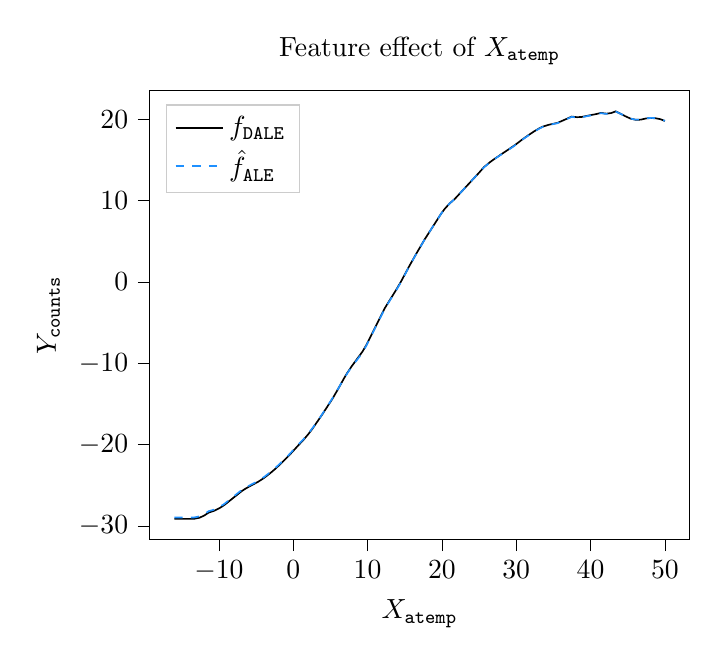
\begin{tikzpicture}

\definecolor{darkgray176}{RGB}{176,176,176}
\definecolor{dodgerblue}{RGB}{30,144,255}
\definecolor{lightgray204}{RGB}{204,204,204}

\begin{axis}[
legend cell align={left},
legend style={
  fill opacity=0.8,
  draw opacity=1,
  text opacity=1,
  at={(0.03,0.97)},
  anchor=north west,
  draw=lightgray204
},
tick align=outside,
tick pos=left,
title={Feature effect of \(\displaystyle X_{\mathtt{atemp}}\)},
x grid style={darkgray176},
xlabel={\(\displaystyle X_{\mathtt{atemp}}\)},
xmin=-19.3, xmax=53.3,
xtick style={color=black},
y grid style={darkgray176},
ylabel={\(\displaystyle Y_{\mathtt{counts}}\)},
ymin=-31.6301535780892, ymax=23.4795271752803,
ytick style={color=black}
]
\addplot [semithick, black]
table {%
-16 -29.1201610565186
-14.5465469360352 -29.1236610412598
-13.3573570251465 -29.1187324523926
-12.6306304931641 -28.9887657165527
-11.9699697494507 -28.7167987823486
-11.3753757476807 -28.351110458374
-10.5825824737549 -28.10817527771
-9.9219217300415 -27.8089466094971
-9.26126098632812 -27.4157428741455
-8.13813781738281 -26.5979690551758
-6.94894886016846 -25.7284774780273
-6.55255270004272 -25.4859237670898
-5.89189195632935 -25.1317119598389
-4.70270252227783 -24.557861328125
-3.90990996360779 -24.0795192718506
-3.11711716651917 -23.5240688323975
-2.52252244949341 -23.0663394927979
-1.86186182498932 -22.5092353820801
-0.540540456771851 -21.3122959136963
0.120120167732239 -20.6509094238281
0.714714765548706 -20.0558643341064
1.30930936336517 -19.4900760650635
2.03603601455688 -18.7049884796143
2.63063073158264 -17.9895362854004
3.8858859539032 -16.3134365081787
5.27327346801758 -14.3682708740234
6 -13.2194204330444
6.85885906219482 -11.8082704544067
7.25525522232056 -11.203857421875
7.91591596603394 -10.3020009994507
9.30330371856689 -8.58228397369385
9.83183193206787 -7.77181529998779
10.9549551010132 -5.72904586791992
12.342342376709 -3.19349336624146
12.5405406951904 -2.89349699020386
13.7957954406738 -1.05008816719055
14.4564561843872 -0.0256915092468262
15.6456460952759 2.00035262107849
16.5705699920654 3.49347949028015
17.6936931610107 5.24578619003296
19.9399394989014 8.44653511047363
20.4024028778076 9.01027202606201
21.0630626678467 9.66129207611084
21.7237243652344 10.1941547393799
24.8948955535889 13.3221054077148
25.687686920166 14.134651184082
26.4804801940918 14.7308025360107
27.1411418914795 15.1683645248413
29.8498497009277 16.8362903594971
30.7087078094482 17.4392356872559
31.3693695068359 17.8697376251221
32.3603591918945 18.484224319458
33.087085723877 18.8724536895752
33.5495491027832 19.0880432128906
34.4084091186523 19.3274822235107
35.0690689086914 19.4596900939941
35.5315322875977 19.543493270874
36.9849853515625 20.1296157836914
37.4474487304688 20.3274917602539
37.6456451416016 20.3095550537109
38.1741752624512 20.2521419525146
38.8348350524902 20.287296295166
39.8258247375488 20.4710922241211
40.6186180114746 20.6114158630371
41.345344543457 20.7675323486328
41.4114112854004 20.7821464538574
41.8078079223633 20.7240734100342
42.1381378173828 20.6876392364502
42.7987976074219 20.7667903900146
43.3933944702148 20.9745426177979
43.657657623291 20.8512020111084
44.714714050293 20.3551597595215
45.4414405822754 20.057201385498
46.1021003723145 19.9324207305908
46.7627639770508 19.9523639678955
47.4894905090332 20.1014881134033
48.1501502990723 20.1500225067139
48.8108100891113 20.1130447387695
49.4054069519043 20.0048065185547
50 19.7889881134033
};
\addlegendentry{$f_{\mathtt{DALE}}$}
\addplot [semithick, dodgerblue, dashed]
table {%
-16 -28.9542388916016
-14.5465469360352 -28.9578762054443
-13.3573570251465 -28.9526977539062
-12.6306304931641 -28.8202018737793
-11.9699697494507 -28.5466842651367
-11.3753757476807 -28.1803741455078
-10.6486482620239 -27.9906787872314
-9.98798751831055 -27.7104911804199
-9.26126098632812 -27.2779521942139
-8.00600624084473 -26.3645648956299
-7.2132134437561 -25.7814712524414
-6.55255270004272 -25.3670864105225
-5.89189195632935 -25.0190086364746
-4.76876878738403 -24.4896812438965
-3.90990996360779 -23.9704494476318
-3.05105113983154 -23.364631652832
-2.52252244949341 -22.9567375183105
-1.86186182498932 -22.4021339416504
-0.606606602668762 -21.2720623016357
0.120120167732239 -20.5483741760254
0.648648619651794 -20.0188083648682
1.30930936336517 -19.4072608947754
1.96996998786926 -18.7101631164551
2.69669675827026 -17.8467922210693
3.55555558204651 -16.7303333282471
4.21621608734131 -15.8174858093262
5.53753757476807 -13.9267387390137
6 -13.1932601928711
6.66066074371338 -12.1299390792847
7.32132148742676 -11.1632461547852
7.91591596603394 -10.3738870620728
8.97297286987305 -9.1130838394165
9.10510540008545 -8.9506664276123
9.83183193206787 -7.83912706375122
11.2852849960327 -5.17018270492554
12.408408164978 -3.13905572891235
13.5975971221924 -1.41476833820343
14.3243246078491 -0.306623458862305
14.6546545028687 0.264089107513428
15.6456460952759 1.96240651607513
16.5705699920654 3.46715188026428
17.6936931610107 5.24065256118774
19.8738746643066 8.35614967346191
20.4024028778076 9.0117301940918
21.0630626678467 9.66457653045654
21.7237243652344 10.1938533782959
25.4894886016846 13.9263477325439
25.6216220855713 14.053521156311
26.4804801940918 14.7064094543457
27.1411418914795 15.1473188400269
29.057056427002 16.3006134033203
29.6516513824463 16.6701507568359
30.6426429748535 17.3715686798096
31.2372379302979 17.7557601928711
32.4924926757812 18.524055480957
33.087085723877 18.8392581939697
33.5495491027832 19.0558605194092
34.4084091186523 19.2951412200928
35.0690689086914 19.4283008575439
35.5315322875977 19.5130195617676
36.9849853515625 20.0959377288818
37.4474487304688 20.291877746582
37.6456451416016 20.2738914489746
38.1741752624512 20.216480255127
38.8348350524902 20.2516288757324
39.8258247375488 20.4354114532471
40.6186180114746 20.5759296417236
41.2792778015137 20.7178859710693
41.4114112854004 20.7472190856934
41.8078079223633 20.6907978057861
42.1381378173828 20.6556282043457
42.7987976074219 20.7358493804932
43.3933944702148 20.9432563781738
43.657657623291 20.8323345184326
45.375373840332 20.0885391235352
46.0360374450684 19.9492740631104
46.6966972351074 19.9548187255859
47.5555572509766 20.1251811981201
48.1501502990723 20.1673374176025
48.8108100891113 20.1304454803467
49.4054069519043 20.0222206115723
50 19.8063983917236
};
\addlegendentry{$\hat{f}_{\mathtt{ALE}}$}
\end{axis}

\end{tikzpicture}
}\\
      (a) & (b) & (c) & (d)
    \end{tabular}
  \end{center}
  \caption{Plot (a): DALE vs ALE execution time on the bike-sharing
    dataset. Plots (b), (c), (d): DALE vs ALE approximation for
    features
    \(X_{\mathtt{month}}, X_{\mathtt{hour}}, X_{\mathtt{atemp}}\)}
  \label{fig:bike-sharing-comparison}
\end{figure}

\begin{table}
  \centering
  \begin{tabular}{c|c|c|c|c}
    \multicolumn{5}{c}{Accuracy} \\
    \hline \hline
    & & \multicolumn{3}{|c}{Number of bins} \\
    \hline
    & & 100 & 50 & 25 \\
    \hline
    \hline
    \multirow{3}{*}{\(X_3\)} & \(\mathtt{NMSE}\) & - & - & - \\
    & \(\mathtt{MSE}\) & - & - & - \\
    & \(\mathtt{VAR}\) & - & - & - \\
    \hline
    \multirow{3}{*}{\(X_6\)} & \(\mathtt{NMSE}\) & - & - & - \\
    & \(\mathtt{MSE}\) & - & - & - \\
    & \(\mathtt{VAR}\) & - & - & - \\
    \hline
  \end{tabular}
  \caption{Evaluation of the divergence between DALE and ALE
    estimation on the Bike Sharing dataset.}
  \label{tab:bike-sharing-accuracy}
\end{table}


% We draw the feature effect plots using K = 100 bins for both
% ALE and DALE.~In Figure~\ref{fig:bike-sharing}, we illustrate
% some of the effects. In almost all cases, both approximations provide
% similar feature effect plots. This confirms our claim that, in cases
% of enough training samples, both methods lead to almost identical
% estimations. This is the case in the bike-sharing dataset where the
% examples cover sufficiently the axis of each attribute. In terms of
% computational speed, DALE approximations is more than \(10\) times
% faster compared to ALE, confirming the notable speed-up even in cases
% with low-dimensional input space.

\message{ !name(5-2-real-datasets.tex) !offset(-135) }
